\documentclass[11pt]{report}
%\usepackage{fullpage}
\usepackage{graphicx}
\usepackage{setspace}
\usepackage[font=small]{caption}
\usepackage{url}

\onehalfspacing
\setlength{\parskip}{0.3cm}

% type user-defined commands here

\begin{document}

\title{CNO: An Attackers Strategy \\
	\vspace{14pt}
	\large UNSW --- ZEIT8020 \\
	Semester 2, 2018
}
\author{Benjamin Simmonds}
\date{September 18, 2018}
\maketitle

\begin{abstract}
	This paper discusses the motivations behind computer network exploitation, the general lifecycle of an attack operation, and the frictions and asymmetries that exist between both the attacker and the defender. One of the greatest challenges is fitting the ever-increasing and changing amount of information into a whole plan or framework to develop the right strategies to prevent such attacks. Armed with this knowledge seek out the creation of a structured general purpose framework for developing offensive strategies, the components described within it, its design philosophy, and how it can be used. It is meant to provide a concrete and structured approach to CNO strategy development.

	This paper considers the various approaches and tools that have proven to be effective, and the resources needed to execute them. By gaining an appreciation of the general principles in the problem space, looking beyond the specifics of industry incidents, attempts distills a generalised framework that is durable and comprehensive. To understand the failure of computer security, one must move beyond analysing a specific event to understanding the inherent characteristics of computer operations. To craft an effective offensive network attack strategy, it is recommended:

	\begin{itemize}
		\item That it be \textit{goal} oriented
		\item That the influences of the \textit{foundational principles} of CNE (humanity, access and economy) on the  operation be considered throughout.
		\item That the uncertainty of \textit{frictions} be minimised, while increasing them for the opponent. If a simple mistake has the potential to kill an operation, the strategy is brittle.
		\item That advantageous \textit{attributes} of the offense be amplified, whilst reducing the beneficial defense  attributes of the opponent.
		\item That the broad perspectives or principles of CNE be evaluated, specifically these include knowledge, awareness, innovation, precaution, operational security and program security.
	\end{itemize}

	In conclusion the paper explores each of the recommendations individually, and provides a suggested set of consideration points, that will aid an organisation in the development of a concrete and opinionated CNO strategy.
\end{abstract}




\chapter{CNE Distilled}


\section{Introduction}
As the volume of security penetrations of companies and government agencies is on the rise, given the ever changing and complex nature of the field of computer operations, postmortem analysis of specific tactics used is not effective, or long lasting.  Consider the methods, strategies and technologies of attacking or defending computer operations, and what hope.

Computer and information systems are as pervasive as ever throughout most aspects of the global economy. The more visible of these such as the Internet, the web, social networking and email often take the lion’s share of generalist media attention, however contemplating the less visible of these systems you get a sense of how significant the ever increasing network of computers and electronic devices has grown; inventory management systems, traffic control systems and internet of things (IoT) devices.

Given the massive economic and  military related implications of information superiority, it is only logical that the art of computer information theft is in high demand, and for some, even a highly paid full time profession, often funded by Governments for national interests. The following chart, prepared by the National Institute of Standards and Technology (NIST, 2018) \cite{nist} highlights the consistent rise in volume and sophistication of attacks.

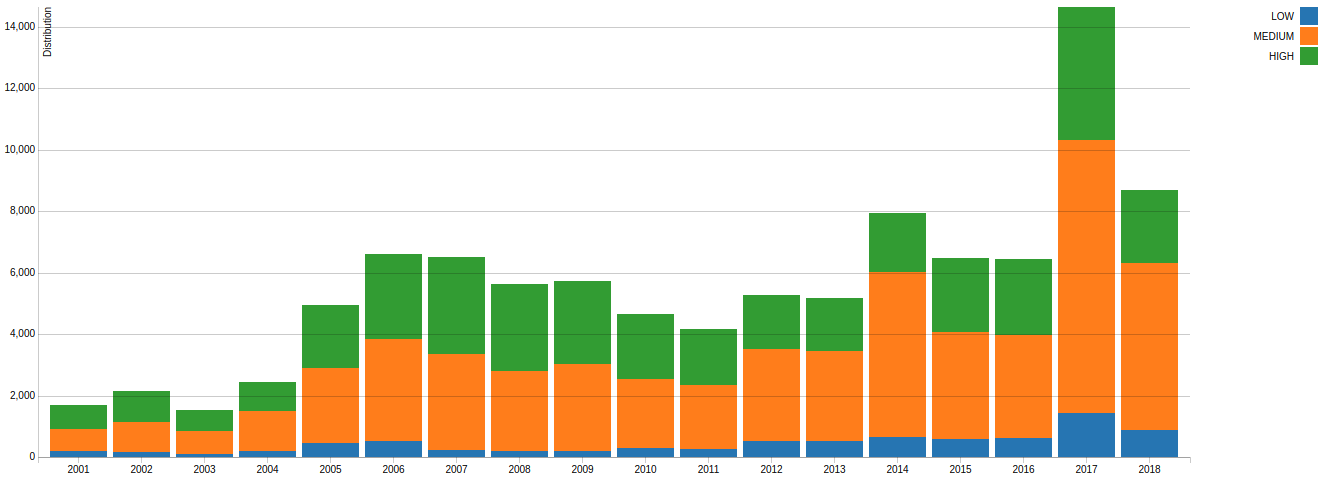
\includegraphics[width=330px]{nist.png}

\begingroup %captionof messes with paragraph indenting if not contained in group
\captionof{figure}{Vulnerabilities Over Time (NIST 2018)}
\endgroup

In a military context, this problem space is more broadly referred to as Computer Network Operations (CNO). CNO is about identifying such cyber-based attacks targeted against your information technology infrastructure, which is typically motivated by human endeavor or warfare through information superiority. This is achieved through a process of data integration and data function of security related information from multiple disparate heterogeneous systems (Bidgoli 2005).

Computer Network Operations encompasses computer network attack (CNA) and computer network defense (CND). The term computer network attack is used to mean the art by which a computer network is subverted via cyber means, whereas the term computer network defense refers to how a computer network is protected from a computer network attack (Blyth \& Kovacich 2001).

Monte (2015, p. 3) \cite{monte} suggests that CNE (Computer Network Exploitation), which is essentially computer espionage, is the key to understanding CNO at large. Truly effective CNA or CND, requires information superiority, whether, in the case of CNA, that be a wider range of access to a target, or in the case of CND, gaining a deeper intuition and understanding of the offense to better craft network defences. In this sense, CNE can be thought of as an enabler of both CNA and CND.



\section{Computer Network Exploitation}

The Department of Defense (Joint Publication 13-3) defines computer network operations (CNO) as: \begin{quote}`` Enabling operations and intelligence collection capabilities conducted through the use of computer networks to gather data from target or adversary automated information systems or networks.''\end{quote}

Distilling the essence of this definition, a CNE operation is one that is highly objective focused, targeted and invisible. All CNE operations and motivations are centered around an objective, for which there could be an infinite number. Monte (2015, p. 5) \cite{monte} generalises these objectives into the following groups:

\begin{itemize}
	\item Strategic collection, is the large scale collection of data over time, which when analysed can highlight further intelligence, such as trends, patterns and capabilities.
	\item Directed collection target the collection of information to meet an immediate objective.
	\item Computer Network Attack (CNA) operations intend to disrupt, deny, degrade or destroy (the four D’s) a target network (e.g. the infamous 2010 “Stuxnet” attack)
	\item Positional access is the targeting of computers and networks that are not directly of interest, but are useful in furthering a greater goal (e.g. computer access of an employee of a target company).
	\item Strategic access, are opportunistic operations that may, or may not, lead to downstream collection or CNA opportunities.
\end{itemize}

Reflecting on the traits that contribute to its success for each of these CNE objective types, endurance is one that clearly stands out. Without endured access, collection efforts are likely to produce poor or no yields, CNA options become severely constrained, usefulness of positional and strategic access computer networks diminishes.

CNE, given its fast moving technological nature, can appear too unwieldy to pin down and frame thinking around. Where does one start? If it were possible to distill the constant everlasting aspects out of CNE, they would serve as excellent building blocks to derive strategies for planning and executing operations, or for defending against those that are. Monte (2015, p. 12) proposes such a system based by considering first principles, principles and themes.

First principles define the fundamental truths. They don’t change.

\begin{itemize}
	\item \textit{Humanity}, refers to the deep human elements that underpin the technology which is ultimately designed, built, used by and monitored by humans.
	\item \textit{Access}, highlights that there is always a method for legitimately accessing target systems and data, otherwise they would not exist in the first place.
	\item \textit{Economy}, drives home that the resources (people, skills, time, money, technology) available to all CNE operations are finite.
\end{itemize}

Principles on the other hand, are not universal, can change over time, but offer a point of view for consideration (Clausewitz 2012). These include topics such as knowledge, awareness, innovation, precaution, operational and program security.

Finally \textit{themes}, \textit{diversity}, \textit{stealth} and redundancy, provide the third and weakest (in terms of durability) level of consideration of CNE, before dropping down to the tactical level.




\subsection{Operation Lifecycle}

Before putting the above generalist consideration framework to use, it is useful to understand how an offensive operation is put together; the various lifecycle stages it consists of and moves through. Bidgoli \& Blyth (Bidgoli 2006, p. 91) present a general purpose CNA model, in which the offence performs  a series of increasingly refined actions on a focused set of  target systems. The model is divided into distinct phases:

\begin{enumerate}
	\item \textit{Targeting}, are the processes used to identify and select  the machines and networks to be penetrated, including the gather of technical (e.g. public networks, software used by the target) and non-technical information (e.g. employees, emails).
	\item \textit{Initial access}, focuses on the activities around gaining access to run shells or software on one the targets computers.
	\item \textit{Exploitation}, are activities that assist in the increase of endured access, the key to  operational success. Including concepts such as persistence and expansion.
	\item \textit{Exfiltration}, is concerned about the smuggling of data out of the target network.
\end{enumerate}

This operation model is high level by design, so that it can be scaled down to more granular activities, allowing it to withstand time as lower level techniques and methods evolve. For example the ATT\&CK framework published by MITRE (MITRE, 2018) defines operational steps that includes:

\begin{enumerate}
	\item Initial Access
	\item Execution
	\item Persistence
	\item Privilege Escalation
	\item Defense Evasion
	\item Credential Access
	\item Discovery
	\item Lateral Movement
	\item Collection
	\item Exfiltration
	\item Command and Control
\end{enumerate}



\subsection{The Offenders Headspace}

By employing first principles, principles and themes, let us conceptualise the offense, or attacker, more closely. This output of this analysis will serve as the foundations for a strategy, that will assist in the prevention (as a defender) or amplification (as an attacker) of an offensive operation.

Ultimately the offence is human, and this humanity drives the objective behind the offensive operations. The motivational factors are varied. Analysis of computer criminals suggests that the primary motivations include the following (Blyth \& Kovacich, 2001; Jones et al., 2002): personal problems, financial gain, peer pressure, and idealism and advocacy.

As an attacker, an awareness of the human element provides focus to the thinking and approaches to the operation at hand. There is a human based objective, every task and action taken should relate to accomplishing the objective. It also is useful to remember that networks, systems and software are all designed and built by humans; flaws, assumptions, shortcuts and all.

``There is always someone with legitimate access and a means to use it'' (Edwards, C \& Kharif, C \& Riley, M 2011). No matter the level of sophistication of security measures put in place, there will be a human that has access to whatever resource the offence is hunting for. It is logical that an attacker should strive to escalate and assume the identity of such a legitimate user. To consider the various access challenges an offender faces, it’s helpful to breakdown the types of connectivity to a network.

\textit{Inbound access}, is a network that enables someone from outside to connect in. Sometimes anonymously, but more commonly restricted by something someone knows (password, SSH key, mouse gesture) or has (e.g. RSA token, mobile phone, email). Attack techniques include impersonation of legitimate identities, leveraging vulnerabilities in exposed network services (e.g. the EternalBlue SMB vulnerability) to inject shellcode and channels for privilege escalation.

\textit{Outbound access}, allows someone from within the network to connect outside the network. More challenging, the attacker needs someone from inside the net to establish a connection out to them. Some examples of attack techniques including email phishing and attached malware, cross site scripting (XSS), website hijack, DNS poisoning, physical media, wireless networks, smartphones and social engineering. Outbound network policies, while common, are in practice porous, due to the friction they create for business users trying to get work done (Monte 2015, p. 34) \cite{monte}.

\textit{Bidirectional access}, a blend of the above inbound and outbound types, is a network that filters, and monitors both inbound and outbound connectivity. Certain services will be available to certain users, and segments on the network.

\textit{No access}, or the ``air gapped'' network. While compared to the other network types, is most secure configuration possible, is no silver bullet. Attack techniques include breaching physical security through fraud, bribe or blackmail (e.g. Stuxnet). The air gap is particularly vulnerable to insider threat (e.g. Snowden).


The offense is burdened with a large amount of technical complexity, often requiring knowledge that is difficult to acquire. A key skill to an effective operation execution, is an awareness of such resource constraints and their management. Cost and Time are the most significant factors, affecting all stages (e.g. targeting or initial access) of an operation. They constrain how thorough any particular stage can go, and the level of investment in offensive capability and expertise. Examples of capability and expertise required for an operation include, multidisciplinary skills related to intelligence acquisition of the target (analysts, linguists, domain experts), exploitation expertise, programmers, hardware engineers, operating system designers, network architects, computing infrastructure and software. On top of specific assets and skill-sets, operational experience and analysts are need to support a well orchestrated operation. An analyst thrives in making informed decisions under pressure, with lots of disconnected pieces of information.



\subsection{Frictions}

Frictions play an important role in the development of an offensive strategy. They are the unpredicted obstructions that slow down or prevent progress in a CNE operation.


\begin{table}[!th]
	\begin{tabular}{ |p{2cm}|p{4.5cm}|p{4.5cm}| }
		\hline
		\textbf{Friction Point} & \textbf{Offensive Examples} & \textbf{Defensive Examples}                                                                                                                                                                                                                                               \\
		\hline
		Mistakes & Target wrong network. Miss vulnerable services. Exfiltrate too much data alerting admins. Miskey IP addresses. & Leave credentials or SSH keys lying around. Mis-configure security or firewalls. Leaving old accounts active.                                                                                         \\
		\hline
		Complexity & Lack of knowledge; network topology, software stacks, user patterns. & Deployment errors, misconfigurations, file systems, protocols, firewalls and network appliances, OS fleet2 managment                                                                                                                          \\
		\hline
		Software & Software is notoriously error prone. Malware and rootkits even more so, due to the specific architecture and OS vulnerabilities they aim to exploit. & Whether through bugs, backdoors, or bad designs, flawed software exists everywhere, a guaranteed constant. Including defensive software such as AV’s and IDP’s. \\
		\hline
		Community & The security community (e.g. Google Project Zero) by bolstering defense, or weakening offense. & End users.                                                                                                                                                                                                           \\
		\hline
		Bad Luck & Hardware failures. Target users go on annual leave. OS patches get rolled out mid operation. & Stolen laptops, disgruntled employees, outages caused by update cycles.                                                                                                                                                 \\
		\hline
	\end{tabular}
	\caption{Friction points from both perspectives}
\end{table}







\chapter{Offensive Strategy}

\section{A Blueprint}

The Concise Oxford Dictionary defines the word strategy as follows: \begin{quote}``A plan of action designed to achieve a long-term or overall aim''\end{quote}

Strategy, not to be confused with tactics, which are the specific actions taken during the execution of a plan. The definitions of the two are often intertwined and clouded, however in the field of CNO, strategy and tactics can be clearly defined from the very moment an attacker obtains initial access. Strategy is everything done in prior to and in preparation for this moment and the resulting operational life cycle that comes into play, whereas tactics represent the actual execution from this point in time onwards.

Strategies must function at the strategic, tactical, and operational levels. At the strategic level, we must focus on developing an understanding of the risks and threats faced both in terms of CND and CNA (Rathmell 2001).

In tactical terms, there is a need to focus on the clear identification of operational procedures and responsibilities, along with system planning and acceptance and business continuity planning (Pfleeger \& Pfleeger 2003). These must be tested and continually revised if they are to be effective.

Drawing the distinction between strategy and tactics, helps frame lower level “tactical” thinking (e.g. specific actions or technologies) which does not tend to endure time well, away from bigger picture long game “strategic” thinking, such as investments in research and development (R\&D) programs or identifying where disaster recovery makes sense or is wasteful.

The key ingredients of a successful CNE strategy are (Monte 2015, p. 93) \cite{monte}:


\begin{itemize}
	\item Being goal oriented.
	\item Understanding the influences of the foundational principles of CNE on the  operation; humanity, access and economy.
	\item Reducing the uncertainty of frictions, while increasing them for the opponent. If a simple mistake has the potential to kill an operation, the strategy is brittle.
	\item Amplifying advantageous attributes of the offense, and reducing the beneficial defense  attributes of the opponent.
\end{itemize}

Using these key ingredients in combination with the framework of principles, we will consider the construction of a boilerplate offensive strategy, that will aid policy makers on strategic issues regarding cyber capabilities, doctrine, and partnerships. To set the stage of a cohesive offensive strategy, the essence of the offensive operations and the organisation itself that will be conducting them should be clearly defined, such as the political goals and implications of success or failure of an operation. To aid this analysis, the below mind map provides a number of high level facets that could be evaluated:


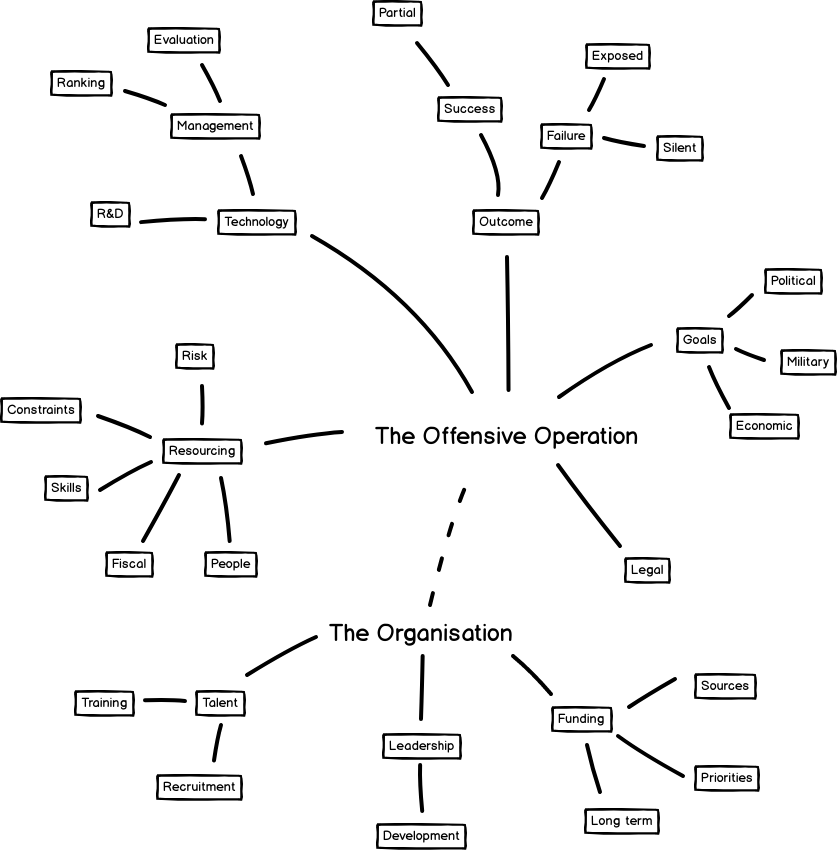
\includegraphics[width=330px]{mindmap.png}

\begingroup %captionof messes with paragraph indenting if not contained in group
\captionof{figure}{Offensive Strategy Ingredients}
\endgroup

To provide depth to the strategy, will consider several perspectives.

The knowledge perspective is concerned with the acquisition and maintenance of knowledge (e.g. technical, psychological). Knowledge is one of the most effective ways of boosting operational performance. As part of an attack strategy, knowledge investment in people, technology and training should be considered from the perspective of the mission, organisation and resources. Some possible considerations include:

\begin{itemize}
	\item What training is needed?
	\item Technical or psychological?
	\item Top 10 technologies that will be encountered?
	\item What knowledge is common to existing or previous operations?
	\item When should technology reuse versus greenfields development occur?
	\item What patterns and/or training programs can be created, to avoid wheel reinvention?
	\item What knowledge is unique, and needs to be carefully guarded?
	\item What methods are used to test that a piece of software can hold up against analysis and detection?
\end{itemize}

The awareness perspective is about raising the level of target specific intelligence, supporting smarter more efficient solutions to problems. This could include having a deep understanding of the opponents network layout, or being alerted to when events of interest occur. In terms of strategy, investment in awareness can be thought of a buying time, which can be funneled into operational activities like data collection, innovation, and redundancy.

\begin{itemize}
	\item How quickly will the opponent organisation likely react?
	\item What’s the fastest reaction time they would need to be effective?
	\item What are the top 10 things to know about the opponent?
	\item How are those things to be monitored?
\end{itemize}

Innovation is about investing in technology, operational techniques and in general fresh ways of thinking. An offensive strategy will balance the investment (resource and budget) in innovation, with measurable real-world applications.

\begin{itemize}
	\item What specific areas of investment would yield the most return on investment (ROI)?
	\item List some assumptions that the defensive industry generally makes.
	\item Would exploiting these channels be beneficial now or in the longer term?
	\item Walkthrough the operational lifecycle from the attackers perspective. Consider strengths and weaknesses (i.e. SWAT analysis) in each stage.
	\item Consider possible research and development (R\&D) funding sources?
	\item What outside research, techniques or technology can be employed?
\end{itemize}

Precaution is all about proactively investing in measures (redundancy and diversity) to prevent something potentially detrimental occuring to an operation. A effective strategy will gauge the level of awareness about the opponent, and if needed fill any gaps by increasing the dosage of redundancy \& diversity applied.

\begin{itemize}
	\item Give technology and approaches planned for an attack operation, what accidental or coincidental actions would jeopardise the operation?
	\item Will you (the attacker) have any visibility into if/when these actions occur? If so, how much time?
	\item Do a risk analysis on each action, by creating a risk matrix. Rank the likelihood and mitigation for each. Estimate a cost for each mitigation.
	\item If a particular problematic defender action arises, how quickly can it be dealt with during the operation. What resources and knowledge is required?
\end{itemize}


The operational security perspective considers insulating an operation from exposure and detection. Some concrete examples of this include limiting the number of technologies deployed as much possible, without putting the operation in jeopardy. Another is considering the approaches that attract the least amount of attention, such as “living of the land” techniques. Operational security is costly, usually requiring investment in knowledge, awareness and innovation. A strategy should aim to strike a good balance, employing the least amount of tactical tradecraft needed to deliver a successful operation.

\begin{itemize}
	\item What is the defensive maturity of the opponent organisation?
	\item How does the investment in precautionary efforts offset operational security?
	\item What is the expected behaviour of the target? How can this be influenced and managed?
	\item Understand your (i.e. the attackers) weakness spots in operational security. For example detection during initial access.
	\item What are the implications on capabilities between avoidance of being seen (stealth) verses simply not being recognised?
\end{itemize}


Lastly program security is focused on the bigger picture of protecting investments and techniques beyond the scope of single operation. In a way it is about maximising the return on investment (ROI), increasing the yields across not just one, but many operations. An offensive strategy will measure the attackers cost of a lost capability, against the cost of the defenders mitigation.

\begin{itemize}
	\item What offensive capabilities does the organisation have (across all operations)? These should be catalogued.
	\item What is the value of each?
	\item What operations have made use of what capabilities and tools?
	\item What synergies exists between operations? What level of reuse or duplication of effort exists?
	\item What level of isolation exists between operations? Would the exposure of the capabilities and methods used in one operation be detrimental to others, and long term investments that have been made?
	\item How are capabilities assigned to operations?
\end{itemize}


\section{Conclusion}

Although CNO remains a fairly immature field, it is clear that new thinking is needed, with change to the typically reactive and lazy ways in which organisations approach computer security at large.

Given the mammoth breadth and depth of technology, its not clear where to start. To appreciate the failure of computer security, elevated thinking above thinking about a specific problem or incident to understanding the inherent characteristics of computer operations.

By drawing out the enduring and foundational aspects of CNO, can better reason about the doctrine, strategies and tactics for executing (or defending) against computer operations.

Through principles and perspectives, have a means for organising analysis and thinking towards the creation of an offensive strategy, typically an overwhelming task due to the sheer breadth and ever changing movement of technology.

The framework presented in this paper raises the signal to noise ratio of computer security strategy, by appreciating the fundamental first principles of CNE; humanity, economy and access, and understanding the traits of the attacker and defender highlight the frictions and assymetries that exists, and in-turn be exploited. Armed with this foundational perspective, can distill offensive principles that are common to all operations; knowledge, awareness, innovation, precaution, operational and program security. Together, forming a framework that can be used to evaluate or develop CNO strategies.



\begin{thebibliography}{9}

	\bibitem{bidgoli}
	Bidgoli, H 2006, Handbook of Information Security, Volume 2, Information Warfare, Social, Legal, and International Issues and Security Foundations, Wiley.

	\bibitem{blyth}
	Blyth, A \& Kovacich, G. L 2001, Information Assurance: Surviving in the Information Environment, 1st ed, Springer-Verlag London

	\bibitem{carr}
	Carr, J 2011, Inside Cyber Warfare: Mapping the Cyber Underworld. O'Reilly Media, Incorporated.

	\bibitem{clausewitz}
	Clausewitz, C., 2012. On War. CreateSpace Independent Publishing Platform.

	\bibitem{edwrds}
	Edwards, C \& Kharif, C \& Riley, M 2011, Human errors fuel hacking as test shows nothing prevents idiocy, accessed 19 August 2018 from bloomberg.com \url{http://www.bloomberg.com/news/articles/2011-06-27/human-errors-fuel-hacking-as-test-shows-nothing-prevents-idiocy}

	\bibitem{defense}
	Joint Publication 13--3, Department of Defense, \url{https://fas.org/irp/doddir/dod/jp3_13.pdf}

	\bibitem{kim}
	Kim, P 2015, The Hacker Playbook 2: Practical Guide To Penetration Testing, CreateSpace Independent Publishing Platform.

	\bibitem{mitre}
	MITRE 2018, ATT\&CK Matrix for Enterprise, accessed 19 August 2018 from mitre.org \url{https://attack.mitre.org/wiki/Main_Page}

	\bibitem{monte}
	Monte, M 2015, Network Attacks and Exploitation: A Framework, Wiley.

	\bibitem{nist}
	NIST 2018, CVSS Severity Distribution Over Time, accessed 19 August 2018 from nist.gov \url{https://nvd.nist.gov/general/visualizations/vulnerability-visualizations/cvss-severity-distribution-over-time#CVSSSeverityOverTime}

	\bibitem{pfleeger}
	Pfleeger, C. P., \& Pfleeger, S. L 2003, Security in computing, 3rd ed, Upper Saddle River, NJ: Prentice Hall.

	\bibitem{rathmell}
	Rathmell, A 2001, Controlling computer network operations. Journal of Information and Security, 7, 121–144.
\end{thebibliography}

\end{document}